\section{Solving parameters using Gauss--Jordan elimination}
Some approaches to solving determined systems of linear equations such as Cramer's rule, require enough constrains to ensure uniqueness of the solution, without it being overdetermined at the same time.
Numerical methods may be difficult to control, and could add additional approximations to the solution.
In our case, the set of available equations is greater than required number of equations that satisfy above conditions.
Out of $2^n$ possible binary vectors representing conditional probability of events, we are forced to pick $n$ that introduce the smallest error in further calculations.
This approach can yield good results when done properly, but the question of which equations to choose remains unanswered.
Preserving linear independence of vectors invokes additional complexity to the rules by which we choose the final set of equations.

Using Gauss--Jordan elimination, we can avoid this problem entirely, since it allows us to work with both overdetermined and underdetermined systems of equations.
The order of equations is also taken into account, so in cases of contradictions, certain combinations are preferred to others.
For the remaining part of this section we will work with linear equations, since using product equations would require us to redefine elementary row operations, thus introducing unnecessary complications.
\subsection{Example of Gauss--Jordan elimination}
Let us propose a simple equation set presented in a standard matrix form $A \cdot X = b$.
\begin{equation}
    \begin{bmatrix}
        1 & 1 & 1 & 0 \\
        1 & 1 & 0 & 0 \\
        0 & 0 & 0 & 1 \\
        0 & 0 & 1 & 0
    \end{bmatrix} \cdot
    \begin{bmatrix}
        x_1 \\ x_2 \\ x_3 \\ x_4
    \end{bmatrix} = 
    \begin{bmatrix}
        b_1 \\ b_2 \\ b_3 \\ b_4
    \end{bmatrix}
\end{equation}

We will use symbols for vector \textbf{$b$}, so we can keep track of operations done on absolute terms.
Turning that into augmented matrix $[A|b]$ yields

\begin{equation}
\begin{bmatrix}[cccc|c]
    1 & 1 & 1 & 0 & b_1 \\ 
    1 & 1 & 0 & 0 & b_2 \\ 
    0 & 0 & 0 & 1 & b_3 \\ 
    0 & 0 & 1 & 0 & b_4
\end{bmatrix}
\end{equation}

Notice that this equation set may be contradictory if we were to use real numbers -- $x_3$ can be calculated as a linear combination of two first rows ($x_3 = b_1 - b_2$) or by taking fourth row as a solution ($x_3 = b_4$).
It is plausible that substituting $b_1$, $b_2$ and $b_3$ with real values calculated from the data file or a database, would lead to $x_3$ being equal to two different numbers.
Additionally, the equation set is underdetermined -- there is not enough information about $x_1$ and $x_2$ to solve them independently.
%Trying to approach that equation set on purely mathematical grounds would lead to quick conclusion that it doesn't make much sense (because of the contradictions).
%Because of the nature of our data and the model, which base on approximations, we allow for certain 

We will now perform Gauss--Jordan elimination steps in order to show that certain properties we care about (such as preserving preference of equations determined by their order) are taken into account.

We will distinguish pivot elements with colors red (currently selected pivot element) and blue (previous pivot elements).
\textbf{During the algorithm we will prefer the topmost pivot element in given column -- this way we assure that topmost equations will be more significant}

\begin{enumerate}
\item We choose the first pivot element (in red), and use it to zero-out remaining coefficients in first column.
\begin{equation}
\begin{bmatrix}[cccc|c]
    \textcolor{red}{1} & 1 & 1 & 0 & b_1 \\ 
    1 & 1 & 0 & 0 & b_2 \\ 
    0 & 0 & 0 & 1 & b_3 \\ 
    0 & 0 & 1 & 0 & b_4
\end{bmatrix}
\begin{matrix} \\ r_2 = r_2 - r_1 \\ \\ \\ \end{matrix} \sim
\begin{bmatrix}[cccc|c]
    \textcolor{blue}{1} & 1 & 1 & 0 & b_1 \\ 
    0 & 0 & -1 & 0 & b_2 - b_1 \\ 
    0 & 0 & 0 & 1 & b_3 \\ 
    0 & 0 & 1 & 0 & b_4
\end{bmatrix}
\end{equation}
\item We select the second pivot element - note that no two pivot elements can share the same row.
The first non-zero element that satisfies this condition is coefficient of $x_3$ in the second row.
\begin{equation}
\begin{bmatrix}[cccc|c]
    \textcolor{blue}{1} & 1 & 1 & 0 & b_1 \\ 
    0 & 0 & \textcolor{red}{-1} & 0 & b_2 - b_1 \\ 
    0 & 0 & 0 & 1 & b_3 \\ 
    0 & 0 & 1 & 0 & b_4
\end{bmatrix}
\begin{matrix} \\ r_2 = r_2 \cdot (-1) \\ \\ \\ \end{matrix} \sim
\begin{bmatrix}[cccc|c]
    \textcolor{blue}{1} & 1 & 1 & 0 & b_1 \\ 
    0 & 0 & \textcolor{red}{1} & 0 & b_1 - b_2 \\ 
    0 & 0 & 0 & 1 & b_3 \\ 
    0 & 0 & 1 & 0 & b_4
\end{bmatrix}
\end{equation}
\begin{equation}
\begin{bmatrix}[cccc|c]
    \textcolor{blue}{1} & 1 & 1 & 0 & b_1 \\ 
    0 & 0 & \textcolor{red}{1} & 0 & b_1 - b_2 \\ 
    0 & 0 & 0 & 1 & b_3 \\ 
    0 & 0 & 1 & 0 & b_4
\end{bmatrix}
\begin{matrix} r_1 = r_1 - r_2\\ \\ \\ r_4 = r_4 - r_2\end{matrix} \sim
\begin{bmatrix}[cccc|c]
    \textcolor{blue}{1} & 1 & 0 & 0 & b_1 - (b_1 - b_2) \\ 
    0 & 0 & \textcolor{blue}{1} & 0 & b_1 - b_2 \\ 
    0 & 0 & 0 & 1 & b_3 \\ 
    0 & 0 & 0 & 0 & b_4 - (b_1 - b_2)
\end{bmatrix}
\end{equation}

\item The last pivot element is going to be coefficient at $x_4$ in the third row.
Since the remaining coefficients are all zeros in fourth column, no changes are made.
We can simplify the values in new vector $b$.
Notice that fourth row is a zero-vector - we can eliminate that from the equation set.
\begin{equation}
\begin{bmatrix}[cccc|c]
    \textcolor{blue}{1} & 1 & 0 & 0 & b_1 - (b_1 - b_2) \\ 
    0 & 0 & \textcolor{blue}{1} & 0 & b_1 - b_2 \\ 
    0 & 0 & 0 & \textcolor{red}{1} & b_3 \\ 
    0 & 0 & 0 & 0 & b_4 - (b_1 - b_2)
\end{bmatrix}
\sim
\begin{bmatrix}[cccc|c]
    \textcolor{blue}{1} & 1 & 0 & 0 & b_2 \\ 
    0 & 0 & \textcolor{blue}{1} & 0 & b_1 - b_2 \\ 
    0 & 0 & 0 & \textcolor{blue}{1} & b_3 \\ 
\end{bmatrix}
\end{equation}
\end{enumerate}

Let us compare our end-result with the initial matrix:
\begin{equation}
\begin{bmatrix}[cccc|c]
    1 & 1 & 1 & 0 & b_1 \\ 
    1 & 1 & 0 & 0 & b_2 \\ 
    0 & 0 & 0 & 1 & b_3 \\ 
    0 & 0 & 1 & 0 & b_4
\end{bmatrix}
\end{equation}

As we can see, $x_3$ was calculated using first and the second row ($b_1 - b_2$).
Let us see what happens after we move the third row on the top position, indicating that our preferred ordering of equations changed. (We expect now to calculate $x_3$ solely by first row).

\begin{enumerate}
\item We choose the our first pivot element, and use it to zero-out remaining coefficients in first column.
\begin{equation}
\begin{bmatrix}[cccc|c]
    0 & 0 & 1 & 0 & b_1 \\
    \textcolor{red}{1} & 1 & 1 & 0 & b_2 \\ 
    1 & 1 & 0 & 0 & b_3 \\ 
    0 & 0 & 0 & 1 & b_4 \\ 
\end{bmatrix}
\begin{matrix} \\ \\ r_3 = r_3 - r_2 \\ \\ \end{matrix} \sim
\begin{bmatrix}[cccc|c]
    0 & 0 & 1 & 0 & b_1 \\
    \textcolor{blue}{1} & 1 & 1 & 0 & b_2 \\ 
    0 & 0 & -1 & 0 & b_3 - b_2 \\ 
    0 & 0 & 0 & 1 & b_1 \\ 
\end{bmatrix}
\end{equation}
\item
Again, no candidate for pivot element in the second column, coefficient at $x_3$ in first row is the next pivot element
\begin{equation}
\begin{bmatrix}[cccc|c]
    0 & 0 & \textcolor{red}{1} & 0 & b_1 \\
    \textcolor{blue}{1} & 1 & 1 & 0 & b_2 \\ 
    0 & 0 & -1 & 0 & b_3 - b_2 \\ 
    0 & 0 & 0 & 1 & b_1 \\ 
\end{bmatrix}
\begin{matrix} \\ r_2 = r_2 - r_1 \\ r_3 = r_3 + r_1 \\ \\ \end{matrix} \sim
\begin{bmatrix}[cccc|c]
    0 & 0 & \textcolor{blue}{1} & 0 & b_1 \\ 
    \textcolor{blue}{1} & 1 & 0 & 0 & b_2-b_1 \\ 
    0 & 0 & 0 & 0 & b_3 - b_2 + b_1 \\ 
    0 & 0 & 0 & 1 & b_4
\end{bmatrix}
\end{equation}
\item Last item fit for a pivot element is a coefficient at $x_4$ in fourth row.
After getting rid of zero vectors, we achieve the following reduced row echelon form matrix
\begin{equation}
\begin{bmatrix}[cccc|c]
    0 & 0 & \textcolor{blue}{1} & 0 & b_1 \\ 
    \textcolor{blue}{1} & 1 & 0 & 0 & b_2-b_1 \\ 
    0 & 0 & 0 & 0 & b_3 - b_2 + b_1 \\ 
    0 & 0 & 0 & \textcolor{red}{1} & b_4
\end{bmatrix}
\sim
\begin{bmatrix}[cccc|c]
    0 & 0 & \textcolor{blue}{1} & 0 & b_1 \\ 
    \textcolor{blue}{1} & 1 & 0 & 0 & b_2-b_1 \\ 
    0 & 0 & 0 & \textcolor{blue}{1} & b_4
\end{bmatrix}
\end{equation}
\end{enumerate}

As expected, $x_3$ was calculated using the most preferred set of equations, as dictated by their order.
What this method does not take into account is the relative weight of each row.
As of yet, all we could rely on was simple ordering of equations, without using the information about quantity or frequency of each type of equation in our learning set.
If our method was to provide that feature to us as well, we could talk about very complete and solid solution that can be expected to perform optimally.

\subsection{Properties of zero vectors}
In this section we will describe how solving the equation set using one order does not prevent us from reproducing other solutions for given parameter.
As we saw previously, different order of equations may lead to different outcomes for certain parameters.
This variety came from contradictions in the equation set.
\begin{description}
\item[Zero vector]\hfill\\
    We will use the term ``zero vector'' to describe the vectors of the form
    \begin{equation}
    \begin{bmatrix}[cccc|c]
        0 & 0 & 0 & 0 & M(b)
    \end{bmatrix},
    \end{equation}
    where $M(b)$ is a linear combination of absolute terms (vector $b$).
\end{description}
Zero vectors that emerge during Gauss--Jordan elimination contain information about other possible solutions for given value.
Instead of removing them in the process, we can store them, and utilize them later.
Let us see how previous example holds to that theory.

\begin{equation}
\begin{bmatrix}[cccc|c]
    1 & 1 & 1 & 0 & b_1 \\ 
    1 & 1 & 0 & 0 & b_2 \\ 
    0 & 0 & 0 & 1 & b_3 \\ 
    0 & 0 & 1 & 0 & b_4
\end{bmatrix}
\sim
\begin{bmatrix}[cccc|c]
    1 & 1 & 0 & 0 & b_1 - (b_1 - b_2) \\ 
    0 & 0 & 1 & 0 & b_1 - b_2 \\ 
    0 & 0 & 0 & 1 & b_3 \\ 
    \textcolor{blue}{0} & \textcolor{blue}{0} & \textcolor{blue}{0} & \textcolor{blue}{0} &\textcolor{blue}{b_4 - (b_1 - b_2)}
\end{bmatrix}
\sim
\begin{bmatrix}[cccc|c]
    \textcolor{blue}{1} & 1 & 0 & 0 & b_2 \\ 
    \textcolor{red}{0} & \textcolor{red}{0} & \textcolor{red}{1} & \textcolor{red}{0} & \textcolor{red}{b_1 - b_2} \\ 
    0 & 0 & 0 & \textcolor{blue}{1} & b_3 \\ 
\end{bmatrix}
\end{equation}

This particular order of equation lead to $x_3$ being calculated from two top-most equations in a set.
If we add our final solution for $x_3$ (vector in red), to the zero vector we ought to remove in a penultimate step of our algorithm (vector in blue), we obtain previously abandoned solution:
\begin{equation}
\begin{bmatrix}[cccc|c]
    0 & 0 & 1 & 0 & b_1-b_2
\end{bmatrix}
+
\begin{bmatrix}[cccc|c]
    0 & 0 & 0 & 0 & b_4 - (b_1 - b_2) \\ 
\end{bmatrix}
=
\begin{bmatrix}[cccc|c]
    0 & 0 & 1 & 0 & b_4
\end{bmatrix}
\end{equation}

Using the same method we can start from the solution obtained after rearranging the order of equations in the initial matrix.
\begin{equation}
\begin{bmatrix}[cccc|c]
    0 & 0 & 1 & 0 & b_1 \\
    1 & 1 & 1 & 0 & b_2 \\ 
    1 & 1 & 0 & 0 & b_3 \\ 
    0 & 0 & 0 & 1 & b_4 \\ 
\end{bmatrix}
\sim
\begin{bmatrix}[cccc|c]
    0 & 0 & 1 & 0 & b_1 \\ 
    1 & 1 & 0 & 0 & b_2-b_1 \\ 
    \textcolor{blue}{0} & \textcolor{blue}{0} & \textcolor{blue}{0} & \textcolor{blue}{0} &\textcolor{blue}{b_3 - b_2 + b_1} \\ 
    0 & 0 & 0 & 1 & b_4
\end{bmatrix}
\sim
\begin{bmatrix}[cccc|c]
    \textcolor{red}{0} & \textcolor{red}{0} & \textcolor{red}{1} & \textcolor{red}{0} &\textcolor{red}{b_1} \\ 
    1 & 1 & 0 & 0 & b_2-b_1 \\ 
    0 & 0 & 0 & 1 & b_4
\end{bmatrix}
\end{equation}

Linear combination of two vectors again yields a different solution

\begin{equation}
\begin{bmatrix}[cccc|c]
    0 & 0 & 1 & 0 & b_1
\end{bmatrix}
+
(-1)\cdot
\begin{bmatrix}[cccc|c]
    0 & 0 & 0 & 0 & b_3 - b_2 + b_1 \\ 
\end{bmatrix}
=
\begin{bmatrix}[cccc|c]
    0 & 0 & 1 & 0 & b_2-b_3
\end{bmatrix}
\end{equation}

Let us look at the example of the equation set with multiple zero vectors:

\begin{equation}
\begin{bmatrix}[cccc|c]
    1 & 1 & 0 & 1 & b_1 \\
    1 & 1 & 0 & 0 & b_2 \\
    0 & 1 & 1 & 0 & b_3 \\ 
    0 & 0 & 1 & 0 & b_4 \\ 
    1 & 0 & 0 & 0 & b_5 \\ 
    1 & 0 & 0 & 1 & b_6 \\ 
\end{bmatrix}
\end{equation}

This equation set is overconstrained -- we can expect to obtain at least two zero vectors after the Gauss--Jordan elimination steps.

\begin{equation}
\begin{bmatrix}[cccc|c]
    1 & 1 & 0 & 1 & b_1 \\
    1 & 1 & 0 & 0 & b_2 \\
    0 & 1 & 1 & 0 & b_3 \\ 
    0 & 0 & 1 & 0 & b_4 \\ 
    1 & 0 & 0 & 0 & b_5 \\ 
    1 & 0 & 0 & 1 & b_6 \\ 
\end{bmatrix} \sim
\begin{bmatrix}[cccc|c]
    1 & 0 & 0 & 0 & b_2 - b_3 + b_4 \\
    0 & 0 & 0 & 1 & b_1 - b_2 \\
    0 & 1 & 0 & 0 & b_3 - b_4 \\ 
    0 & 0 & 1 & 0 & b_4 \\ 
    0 & 0 & 0 & 0 & -b_2 + b_3 - b_4 + b_5 \\ 
    0 & 0 & 0 & 0 & -b_1 + b_3 - b_4 + b_6 \\ 
\end{bmatrix}
\begin{matrix}
v_1 \\ v_2 \\ v_3 \\ v_4 \\ v_5 \\ v_6
\end{matrix}
\label{eq:gauss_jordan1}
\end{equation}

Let us mark each vector in a reduced row echelon form (Equation~\ref{eq:gauss_jordan1}) as $v_1 \ldots v_6$.
As we had shown previously, we can use zero vectors to obtain different solutions to parameters $x_1 \ldots x_4$, for example:

\begin{equation}
\begin{matrix}[cccc|c|c]
    & & & & \mbox{combination} & \mbox{value} \\
    \hline
    [1 & 0 & 0 & 0]_1 & v_1 & b_2-b_3+b_4 \\
    [1 & 0 & 0 & 0]_2 & v_1+v_5 & b_5 \\
    [1 & 0 & 0 & 0]_3 & v_1+v_6 & -b_1 + b_2 + b_6 \\
    \hline
    [0 & 1 & 0 & 0]_1 & v_3 & b_3 - b_4 \\
    [0 & 1 & 0 & 0]_2 & v_3 - v_5 & b_2 - b_5 \\
    [0 & 1 & 0 & 0]_3 & v_3 - v_6 & b_1 - b_6 \\
    \hline
    & & \cdots & & \cdots & \cdots \\
    \hline
    [0 & 0 & 0 & 1]_1 & v_2 & b_1 - b_2 \\
    [0 & 0 & 0 & 1]_2 & \textcolor{red}{v_2  + v_6 - v_5}& b_6 - b_5 \\
    \hline
    & & \cdots & & \cdots & \cdots \\
\end{matrix}
\end{equation}

Notice that the second solution for $x_4$ (in red above) requires two zero vectors to find an efficient solution.

We would like to propose a conjecture describing relationship of possible solutions with zero vectors in reduced row echelon form matrix.
\begin{description}
	\item[Zero-vector conjecture] \hfill \\
        Every possible solution for given parameter $q$ can be obtained as a linear combination of a solution vector from Gauss--Jordan elimination, and the zero vectors, i.e.,
    {\large
    \begin{equation}
    \begin{matrix}
        \forall_{s \in S} \displaystyle\exists_{a \in V} \; s = [1,a_1,a_2,\ldots,a_n]\cdot[s_0,z_1,z_2,\ldots,z_n]=\\=s_0 + a_1 \cdot z_1 + a_2 \cdot z_2 +\cdots+a_n \cdot z_n
    \end{matrix}
    \end{equation}
    }
    where $s \in S$ is a solution vector $s$ for parameter $q$ from a space of all possible solutions $S$ \\
    $a \in V$ is the vector of coefficients from a vector space $V$ over a field $\mathbb{R}$ \\
    $s_0$ is the first solution (also a vector over a field $\mathbb{R}$) for given parameter, as obtained from Gauss--Jordan elimination \\
    $z_i$ is the $i$-th zero vector obtained from Gauss--Jordan elimination ($i \in 1\ldots n$). \\
    $n$ is the number of zero vectors in reduced row echelon form.
	\item[Proof] \hfill \\
    If the equation set is determined, each parameter has a unique solution. Since in that case there are no zero vectors, $n=0 => s = [1] \cdot [s_0] = s_0$.\\
    Similar case would emerge when the equation set is strictly underdetermined (not every parameter has a unique solution, but no zero vectors appear in reduced row echelon form either).
    Third case would be equation sets with over-constrainments, which are of our interest here since they produce zero vectors after Gauss--Jordan elimination.

    First, let's define two terms we will later use:

    \begin{description}
    	\item[Linear combination of equation set] \hfill \\
            Linear combination of the equation set can be interpreted as a function
            {\large
            \begin{equation}
                f: \mathbb{M}_{m \times n} \to \mathbb{M}_{m \times n}
            \end{equation}
            }

            where $\mathbb{M}_{m \times n}$ is a space of matrices of size $m \times n$.

            Additionally every such function $f$ is equivalent to left multiplication by some matrix $F$,~that is
            {\large 
            \begin{equation}
                \forall_{f} \forall_{A_0 \in \mathbb{M}_{m \times n}} \exists_{F \in \mathbb{M}_{m \times m}} \; f(A_0) = F \cdot A_0
            \end{equation}
            }

            Example: Equivalence relation~\ref{eq:gauss_jordan1} could also be written as an equation:
            \begin{equation}
            \begin{bmatrix}
                0 & 1 & -1 & 1 & 0 & 0 \\
                1 & -1 & 0 & 0 & 0 & 0 \\
                0 & 0 & 1 & -1 & 0 & 0 \\ 
                0 & 0 & 0 & 1 & 0 & 0 \\ 
                0 & -1 & 1 & -1 & 1 & 0 \\ 
                -1 & 0 & 1 & -1 & 0 & 1 \\ 
            \end{bmatrix} \cdot
            \begin{bmatrix}[cccc|c]
                1 & 1 & 0 & 1 & b_1 \\
                1 & 1 & 0 & 0 & b_2 \\
                0 & 1 & 1 & 0 & b_3 \\ 
                0 & 0 & 1 & 0 & b_4 \\ 
                1 & 0 & 0 & 0 & b_5 \\ 
                1 & 0 & 0 & 1 & b_6 \\ 
            \end{bmatrix} =
            \begin{bmatrix}[cccc|c]
                1 & 0 & 0 & 0 & b_2 - b_3 + b_4 \\
                0 & 0 & 0 & 1 & b_1 - b_2 \\
                0 & 1 & 0 & 0 & b_3 - b_4 \\ 
                0 & 0 & 1 & 0 & b_4 \\ 
                0 & 0 & 0 & 0 & -b_2 + b_3 - b_4 + b_5 \\ 
                0 & 0 & 0 & 0 & -b_1 + b_3 - b_4 + b_6 \\ 
            \end{bmatrix}
            \begin{matrix}
            v_1 \\ v_2 \\ v_3 \\ v_4 \\ v_5 \\ v_6
            \end{matrix}
            \label{eq:gauss_jordan2}
            \end{equation}
            in which case the leftmost matrix would be our linear combination of Gauss--Jordan elimination algorithm.

        \item[Solution vector] \hfill \\
            Solution vector is a single row in a matrix (usually obtained by linear combination of the equation set), directly solving given parameter $x_k$ (vector $[\;0 \;\ldots\;0\;1\;0\; \ldots 0 \;|\; b\;]$ with ``$1$'' at the $k$-th place, and some absolute term $b$ in its augmented form).

            Example:
            Row $v_2$ in equation~\ref{eq:gauss_jordan2} unambiguously gives solution to parameter $x_4$, thus vector $[\;0\;0\;0\;1\;|\;b_1 - b_2\;]$ is the solution vector of $x_4$.
    \end{description}

    We will now prove the conjecture in question. 

    Let $\boldsymbol{A}$ be the original equation set, and $\boldsymbol{B}$ - the equation set after Gauss--Jordan elimination (reduced row echelon form).
    Let us say that given parameter $x_m$ can be calculated using at least two different linear combinations of vectors from $\boldsymbol{A}$.
    Let us call these $L_0$ and $L_k$, where $L_0$ is linear combination equivalent to Gauss--Jordan elimination ($\boldsymbol{B} = L_0 \cdot \boldsymbol{A}$).
    Let us assume that $s_0$ is the solution vector for parameter $x_m$ as obtained from Gauss--Jordan elimination (that is $s_0 \in \boldsymbol{B}$)

    $s_0$ is a solution vector in in $\boldsymbol{B}$.

    $s_k$ is a solution vector in $L_k \cdot \boldsymbol{A}$, but it is not a vector in $\boldsymbol{B}$.
    %(otherwise we would have linearly dependent non-zero vectors in $\boldsymbol{B}$ which does not happen after Gauss--Jordan elimination steps).

    We can show that $s_k$ can also be obtained as linear combination of vectors from $\boldsymbol{B}$ using only $s_0$ and the zero vectors, by splitting the conjecture into two parts:
    \begin{enumerate}
    \item Vector $s_k$ can be obtained as a linear combination of vectors from $\boldsymbol{B}$: \hfill \\
        Since $L_0$ is determined by Gauss--Jordan elimination, which in turn uses only elementary row operations, $L_0$ is an invertible matrix.
        Thus $L_0^{-1}$ exists. Because $L_0^{-1} \cdot L_0 = \mbox{Id}$, and matrix multiplication is associative, we can apply the following:
        \begin{equation}
        \begin{matrix}
            s_k \in L_k \cdot \boldsymbol{A} \Rightarrow s_k \in L_k \cdot (L_0^{-1} \cdot L_0) \cdot \boldsymbol{A} \Rightarrow s_k \in L_k \cdot L_0^{-1} \cdot \boldsymbol{B}
        \end{matrix}
        \end{equation}
        Because $s_k$ is a vector in $L_k \cdot \boldsymbol{A}$ then $s_k$ is also a vector in $L_k \cdot L_0^{-1} \cdot \boldsymbol{B}$.
        In that case we can use a linear combination $L_k \cdot L_0^{-1}$ to go from solution $s_0$ to $s_k$.

    \item Vector $s_k$ in $L_k \cdot L_0^{-1} \cdot \boldsymbol{B}$ is a linear combination of vectors no other than $s_0$ and the zero vectors in $\boldsymbol{B}$:\hfill \\
        \textcolor{red}{(Quite hand-wavy argument I'm not satisfied with yet)}

        Because $\boldsymbol{B}$ is a reduced row echelon form, the following property holds: no two non-zero coefficients in reduced row echelon form share the same column.

        Let us assume that vector $s_k$ is calculated using two non-zero vectors in its linear combination from $\boldsymbol{B}$ to $L_k \cdot \boldsymbol{A}$.
        In that case, $s_0$ has to appear in a linear combination with a non-zero coefficient since no other non-zero vector can produce a $1$ in $m$-th column in $s_k$.
        Additionally, any linear combination involving any two non-zero vectors from $\boldsymbol{B}$ with both coefficients other than $0$ will produce a vector with at least two coefficients other than $0$.
        Such vector would not be a solution vector, which $s_k$ is. Contradiction.
        %$\Rightarrow$ coefficients at non-zero vectors other than $s_0$ in $s_k \in L_k \cdot L_0^{-1}$ have to be $0$.
    \end{enumerate}
\end{description}

Finding such linear combination is no trivial task.
The solution space is infinite, and virtually any linear combination of zero vectors can be added to any non-zero vector, giving us an valid solution (although the combination would be very inefficient in most cases)

\subsection{Modifying systems of equations}
In previous sections we showed that we can use Gauss-Jordan elimination to explore space of solution for each parameter in fairly controlled environment.
We have to remember however that our equations are not standard linear equations, but product equations.
By product equations we mean equations such~as
\begin{equation}
    1 - (1-p_1)\cdot(1-p_2) \cdots (1-p_n) = b_k.\\
\end{equation}
%where $p_i$ is the probability of $i$-th parent node activating the child node in question, with all other causes being not present (FIXME: UGLY), and $b_k$ is conditional probability of given events taking place.
In order to simplify the equation, we introduce substitutions $\forall_kq_k = 1 - p_k$ and $c_k = 1 - b_k$.
This gives us equation of form
\begin{equation}
    q_1 \cdot q_2 \cdots q_n = c_k.
\end{equation}
Of course not every cause is present in given case, resulting in some parameters not taking part in the product on the left side of the equation.
Let us propose an example of such equation:
\begin{equation}
\begin{cases}
    1 - (1-p_1) \cdot (1-p_2) \cdot (1-p_3) \cdot (1-p_4) &= b_1\\
    1 - (1-p_3) \cdot (1-p_4) & = b_2\\
    1 - (1-p_1) \cdot (1-p_2) \cdot (1-p_4) & = b_3\\
    1 - (1-p_3) & = b_4\\
\end{cases}
\sim
\begin{cases}
    q_1 \cdot q_2 \cdot q_3 \cdot q_4 &= c_1\\
    q_3 \cdot q_4 &= c_2\\
    q_1 \cdot q_2 \cdot q_4 &= c_3\\
    q_3 &= c_4\\
\end{cases}.
\end{equation}

Taking logarithm of both sides yields the following system:
\begin{equation}
\begin{cases}
    log_p{q_1} + log_p{q_2} + log_p{q_3} + log_p{q_4} &= log_p{c_1}\\
    log_p{q_3} + log_p{q_4} &= log_p{c_2}\\
    log_p{q_1} + log_p{q_2} + log_p{q_4} &= log_p{c_3}\\
    log_p{q_3} &= log_p{c_4}\\
\end{cases}.
\end{equation}

Since this gives us a linear equation set, Gauss--Jordan elimination is applicable.
\subsection{Eliciting leak parameter}
In this section we will discuss our approach to eliciting leak parameter from the data file.
Since leak is slightly different from ordinary parameters, we have to approach this endeavour with high cautious.
Leak, when not expressed explicitly in the data file, is represented in the probability of all parent nodes being in the distinguished state with child node being activated.
%%\begin{figure}[h!]
%    \begin{center}
%     \noindent\begin{minipage}{.5\linewidth}%
%        \begin{tikzpicture}[scale=1.5]
%        \tikzstyle{vertex}=[draw,text=black,auto=left,circle,fill=white,minimum size=25pt]
%        \tikzstyle{blank}=[draw,color=white,text=black,auto=left,circle,fill=white,minimum size=25pt]
%        \node[vertex] (P1) at (1, 0) {$P_1$};
%        \node[vertex] (P2) at (1.8, 0) {$P_2$};
%        \node[vertex] (P3) at (2.6, 0) {$P_3$};
%        \node[blank] (dots) at (3.2, 0) {$\cdots$};
%        \node[vertex] (P4) at (3.8, 0) {$P_n$};
%        \node[vertex] (C) at (2.6, -1) {C};
%  
%        \foreach \from/\to in {P1/C, P2/C, P3/C, P4/C}
%        \draw[->, >=latex] (\from) -- (\to);
%
%        \end{tikzpicture}
%        \caption{Simple Bayesian Network}
%        \label{graph:bn1}
%
%    \end{minipage}%
%    \begin{minipage}{.5\linewidth}
%\begin{tabular}{|l|l|l|l|l|l|}
%    
%    \hline
%    Prior & $Q_1$ & $Q_2$ & $Q_3$ & $\ldots$ & $Q_n$ \\
%    \hline
%    $P(Q_k,+)$ & $0.9$ & $0.9$ & $0.9$ & $\ldots$ & $0.9$ \\
%    $P(Q_k,-)$ & $0.1$ & $0.1$ & $0.1$ & $\ldots$ & $0.1$ \\
%    \hline
%\end{tabular}
%
%\end{minipage}
%
%    \end{center}
%    hello
%%\end{figure}
%%

\begin{figure}[!ht]
  \begin{subfigure}[b]{.5\linewidth}
    \centering
        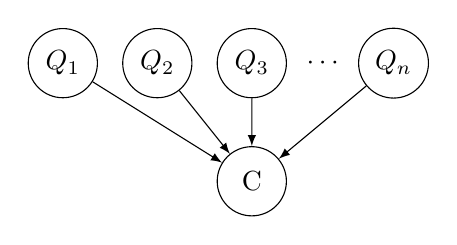
\begin{tikzpicture}[scale=1.5]
        \tikzstyle{vertex}=[draw,text=black,auto=left,circle,fill=white,minimum size=25pt]
        \tikzstyle{blank}=[draw,color=white,text=black,auto=left,circle,fill=white,minimum size=25pt]
        \node[vertex] (P1) at (1, 0) {$Q_1$};
        \node[vertex] (P2) at (1.8, 0) {$Q_2$};
        \node[vertex] (P3) at (2.6, 0) {$Q_3$};
        \node[blank] (dots) at (3.2, 0) {$\cdots$};
        \node[vertex] (P4) at (3.8, 0) {$Q_n$};
        \node[vertex] (C) at (2.6, -1) {C};
  
        \foreach \from/\to in {P1/C, P2/C, P3/C, P4/C}
        \draw[->, >=latex] (\from) -- (\to);
        \end{tikzpicture}
    \caption{Structure of simple Bayesian Network}
    \label{graph:bn1}
  \end{subfigure}%
  \begin{subfigure}[b]{.5\linewidth}
    \centering
\begin{tabular}{|c|c|c|c|c|c|}
    
    \hline
        & $Q_1$ & $Q_2$ & $Q_3$ & $\ldots$ & $Q_n$ \\
    \hline
    $P(Q_k=+)$ & $p_1$ & $p_2$ & $p_3$ & $\ldots$ & $p_n$ \\\hline
    $P(Q_k=-)$ & $1-p_1$ & $1-p_2$ & $1-p_3$ & $\ldots$ & $1-p_n$ \\\hline
\end{tabular}

    \subcaption{Prior probability of parent nodes}
    \label{table:bn1}
  \end{subfigure}
  %\caption{A figure with two subfigures}
  %\label{fig:1}
\end{figure}
Let us assume that prior probability of parents $Q_1, \cdots, Q_n$ (see Figure~\ref{graph:bn1}) being in the distinguished stated is $(1-p_1), \cdots, (1-p_n)$ respectively.
In that case, incidence of vector describing leak within the data file is equal to:
\begin{equation}
    \prod_{i=1}^n (1-p_i)
\end{equation}
This is a trivial remark, since similar product can be derived for any combination of parent states.
As we had shown previously, in case of other parameters we can aid our efforts of solving parameters by means of linear combination of vectors and linear algebra.
We would like to achieve similar freedom in solving leak as well.
This is especially important if parameters $p_1 \cdots p_n$ would be relatively high, favoring non-distinguished states to occur more often.
Since in such cases records describing leak can be relatively rare, we can try to express leak as one of the explicit parameters.
For this we will compare two approaches to interpreting leak within the data.
\textcolor{red}{(reference to canonical.pdf - diez and henrion approach to leak)}
\begin{equation}
    P(y|x) = 1 - (1 - p_L) \cdot \prod_{i\in I(x)}(1-p_i)
    \label{eq:diez_leak}
\end{equation}

\begin{equation}
    P(y|x) = 1 - (1 - p_L) \cdot \prod_{i\in I(x)}\frac{1-p'_i}{1-p_L}
    \label{eq:henr_leak}
\end{equation}

Equation~\ref{eq:diez_leak} is the definition of leak by Diez[\textcolor{red}{reference}], while Equation~\ref{eq:henr_leak} is the definition proposed by Henrion[\textcolor{red}{reference}].
We can make a transition between $p_k$ and $p'_k$ for any $k$ using Equation~\ref{eq:henr_diez_trans}.
\begin{equation}
    1-p_k = \frac{1-p'_k}{1-p_L}
    \label{eq:henr_diez_trans}
\end{equation}

Since main concern of our research is learning from data, Henrion's definition is to be applied, but
because it is easy to transition between these, we can explore both ways and choose the one that yields better flexibility.
Let us see how we would approach adding leak to the data:

\begin{table}[h!]
\begin{center}
\begin{tabular}{|l|l|l|l|l|l|l||p{1.5cm}|}
	\hline
	\# & $P_1$ & $P_2$ & $P_3$ & $P_4$ & Leak--Diez & Leak--Henrion & $P(y|x)$ \\\hline
    1 & 1 & 1 & 0 & 0 & 1 & -1 & $p_1$ \\
    2 & 0 & 1 & 1 & 1 & 1 & -2 & $p_2$ \\
    3 & 1 & 1 & 1 & 0 & 1 & -2 & $p_3$ \\
    4 & 0 & 0 & 1 & 0 & 1 & 0 & $p_4$ \\
    5 & 0 & 0 & 0 & 0 & 1 & 1 & $p_5$ \\
    %$\cdots$ & $\cdots$ & $\cdots$ & $\cdots$ & $\cdots$ & $\cdots$ & $\cdots$\\
    \hline
\end{tabular}
	    \caption{Example of data supplemented with explicit leak parameters using both approaches.}
		\label{tab:bn}
\end{center}
\end{table}

Interpreting leak by Diez's definition results in adding a column of ones to the data, indicating that leak was present in every case (this also derives from Equation~\ref{eq:diez_leak}).

The values in the column ``Leak--Henrion'' may be interpreted as exponents of each item in the product.
Negative value $-k$ indicates positive exponent $k$ in the denominator of the product (Equation~\ref{eq:henr_leak}).
This rule still holds after we take logarithm of both sides, since then we treat the values in the data as coefficients of logarithms.

\begin{enumerate}
\item \textbf{Diez's definition:}\hfill\\ 
Algorithm would be performed in three steps:
\begin{enumerate}
    \item Solve the equation set for leak first
    \item Apply transition~\ref{eq:henr_diez_trans} to the original parameters
    \item Solve the original equation (without leak) for each of the parameters
\end{enumerate}
This would yield us the final parameters with leak included, as defined by Henrion.

\item \textbf{Henrion's definition:}\hfill\\
    Since the Equation~\ref{eq:henr_leak} already suits our case of learning from data, solving the equation yields us the final parameters.
\end{enumerate}

It may seem that second approach is simpler and handles the issues with leak for us, since there's no additional step of including leak to initial parameters from Diez's approach.
Yet, since they are equivalent, there's no other way than to agree that potential error in leak will carry on to parameters with both approaches anyway.
In that case, using Henrion's approach to supplement the data with leak is slightly disadvantageous, since it limits our solution for leak to the first solution obtained by Gauss--Jordan elimination.
